\section{Descrizione e schema dell'architettura}
\subsection{Schema}
\begin{figure}[h]
    \centering
    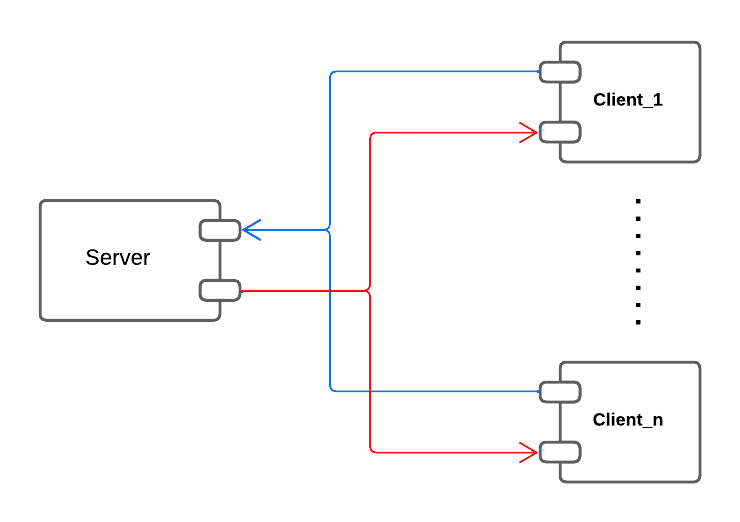
\includegraphics[width=0.8\textwidth]{imagens/schema.png}
    \caption{Schema dell'architettura}
    \label{fig:schema}
\end{figure}

La Figura \ref{fig:schema} mostra la comunicazione tra i vari client ed il server. Il client prevede un writer ed un reader per la lettura e scrittura su socket del server. Il server, al contempo, prevede un writer ed un reader per la lettura e scrittura su socket del client.

\subsection{Architettura}
E' stato optato per \texttt{Java} come linguaggio principale per il suo mix di portabilità, semplicità d'uso e solidità.
Come richiesto, è stata scelta come architettura di comunicazione quella "client/server". L'implementazione di essa è stata resa possibile grazie all'utilizzo delle \texttt{Socket}. 

\subsubsection{Componenti fondamentali}
Si procede di seguito ad elencare i principali componenti dell'applicativo in fase di sviluppo. Essi sono:
\begin{itemize}
    \item \textbf{Client:} risulta essere l'utente che utilizza l'applicativo. E' stata pensata una sola interfaccia (da terminale) per entrambe le tipologie di utenti (Base e Moderatore); in seguito alla connessione verrà stabilito automatichemente il livello di privilegio. In quanto tale, può utilizzare l'applicativo inviando comandi al server e visualizzando il risultato. \newline
    \item \textbf{Server: } accetta le connessioni in entrata e permette l'autenticazione degli utenti. Solo se il nome utente non è già stato utilizzato permette lìaccesso ad esso; altrimenti richiede un'altro nome utente. Solamente dopo l'autenticazione, permette l'esecuzione dei comandi lato server. Riceve i comandi inviati dall'utente e li esegue; se necessario restituisce quanto richiesto dal comando.
\end{itemize}

\subsubsection{Flusso di comunicazione (Server -> Client)}
\begin{enumerate}
    \item Apertura della socket del Server
    \item Ascolto connessioni in entrata
    \item Ascolto messaggi dai client ed esecuzione comandi (Thread)
    \item Chiusura della connessione
\end{enumerate}
Essendo che il server è stato predisposto per accogliere più client e gestirli in maniera concorrente, sono stati predisposti due flussi di esecuzione paralleli, di cui uno è un thread il quale gestisce l'ascolto dei messaggi dai client, per eseguire i comandi utente inviatigli. Il flusso principale di esecuzione gestisce invece le connessioni in arrivo. Più nello specifico, vi è un loop per accogliere le connessioni in entrata, una volta stabilita una connessione, viene fatto partire un thread per tale connessione che ascolterà i messaggi in arrivo dal client specifico.

\subsubsection{Flusso di comunicazione (Client -> Server)}
\begin{enumerate}
    \item Autenticazione al server tramite nome univoco
    \item Accesso al server
    \item Invio comandi al server
    \item Visualizzazione risultato
\end{enumerate}
In questo caso, il client non richiede nessuna particolare azione, se non quella di effettuare l'accesso al server tramite nome univoco. Una volta effettuato l'accesso con successo, esso sarà in grado di eseguire i comandi sul server ed ottenere una risposta.
